% !TEX program = xelatex
%%%%%%%%%%%%%%%%%%%%%%%%

\documentclass[11pt,aspectratio=169]{beamer} % 11pt is default
\usetheme{metropolis} % [progressbar=frametitle]
\setbeamercolor{background canvas}{bg=white}
\setbeamertemplate{caption}{\insertcaption} 
\setbeamersize{text margin left=2em,text margin right=2em}
\setbeamertemplate{frame footer}{\vspace{-5pt}}

\usepackage[round]{natbib}
\usepackage{amsmath}
\usepackage{mathtools}
\usepackage[group-minimum-digits=4,group-separator={,}]{siunitx}
\usepackage{graphicx}
\usepackage{wrapfig}
\usepackage{multimedia}

\usepackage{tikz}
\usetikzlibrary{backgrounds}
\usetikzlibrary{arrows,shapes}
\usetikzlibrary{tikzmark}
\usetikzlibrary{calc}
\usepackage[dvipsnames]{xcolor}

\usepackage[skins,theorems]{tcolorbox}
\usepackage{pdfpages}
\usepackage{colortbl}
\usepackage{changepage}
\usepackage{booktabs}
\usepackage{makecell}
\usepackage{setspace}
\usepackage{algorithm}
\usepackage[noend]{algpseudocode}
\usepackage{subcaption}
\usepackage[framemethod=TikZ]{mdframed}
\usepackage{xspace}

\usepackage{annotate-equations}

% Shortcut for beamer frames
\newcommand{\bframe}[2][c]{\begin{frame}[#1]{#2}}
\newcommand{\eframe}{\end{frame}} % \eframe causes problems for some reason

% Shortcut for bold text
\newcommand{\fat}[1]{\textbf{#1}}

% Boxing items on slide
\newcommand{\Cboxed}[2]{\colorlet{currentcolor}{.}{\color{#1}\fbox{\color{currentcolor}#2}}} %create coloured box around equation

% checkmark and xmark
\usepackage{pifont}
\newcommand{\cmark}{\ding{51}}%
\newcommand{\xmark}{\ding{55}}%

% Highlighting text in orange
\newcommand{\e}[1]{\alert{#1}}

% Underline
\newcommand{\uline}[1]{\underline{#1}}

% Include figure
\newcommand{\imgw}[2]{\includegraphics[width=#2\textwidth]{#1}} % \imgw{file}{height-scale}
\newcommand{\imgh}[2]{\includegraphics[height=#2\textheight]{#1}} % \imgh{file}{width-scale}

% Shortcut for latex commands
\newcommand{\blist}{\vspace{-3pt}\begin{list}{\raisebox{1pt}{\small$\bullet$}}{\leftmargin=13pt\itemsep=4pt}}
\newcommand{\blisttab}{\vspace{5pt}\blist}
\newcommand{\elisttab}{\end{list}}
\newcommand{\listtab}{\\[3pt] $\Rightarrow$ }
\newcommand{\elist}{\end{list}\vspace{5pt}}
\newcommand{\bblock}[1]{\metroset{block=fill}\begin{block}{#1}}
\newcommand{\eblock}{\end{block}}
\newcommand{\bmath}[1][0]{\begin{equation*}\hspace{#1em}}
\newcommand{\emath}{\end{equation*}}
\newcommand{\bcol}{\begin{columns}}
\newcommand{\col}[1]{\column{#1\textwidth}}
\newcommand{\tcol}[1]{\column[T]{#1\textwidth}}
\newcommand{\ecol}{\end{columns}}
\newcommand{\place}[4]{\begin{textblock}{#3}(#1,#2) #4 \end{textblock}} % \place{x}{y}{width}{text}
\newcommand{\placeframed}[4]{\place{#1}{#2}{#3}{\fbox{\parbox{#3em}{#4}}}}
\newcommand{\placeimg}[4]{\place{#1}{#2}{#3}{\imgw{#4}{1}}} % \placeimg{x}{y}{width}{file}
\newcommand{\videolink}[2]{\movie[externalviewer]{{\bf Video:} #1}{videos/#2}} % \videolink{title}{file}
\newcommand{\btab}[1]{\begin{tabular}{#1}}
\newcommand{\etab}{\end{tabular}}
\newcommand{\balgo}[2][1.3]{{#2:} \\[5pt] \begin{algorithmic}[1] \linespread{#1}\selectfont}
\newcommand{\ealgo}{\end{algorithmic}}
\renewcommand{\algorithmicloop}{\textbf{repeat:}}
\newcommand{\cred}{\cellcolor{red!25}}
\newcommand{\cgreen}{\cellcolor{green!25}}

% Shortcut for commonly used math symbols
\newcommand{\condpr}[2]{\text{Pr}\hspace{-1pt}\left\{ #1 \ \mid \ #2 \right\}}
\newcommand{\exarg}[2]{\mathbb{E}_{#1}\hspace{-2pt}\left[ #2 \right]}
\newcommand{\exnoarg}[1]{\mathbb{E}_{#1}}
\NewDocumentCommand\ex{ m g }{
	\IfNoValueTF{#2}{\exnoarg{#1}}{\exarg{#1}{#2}}
}
\newcommand{\der}[2]{\frac{\partial #1}{\partial #2}}
\newcommand{\stats}{\mathcal{S}}
\newcommand{\acts}{\mathcal{A}}
\newcommand{\rews}{\mathcal{R}}
\newcommand{\eps}{\mathcal{E}}
\newcommand{\ver}{\,\vert\,}
\newcommand{\vhat}{\hat{v}}
\newcommand{\qhat}{\hat{q}}
% \newcommand{\para}{\textbf{w}}
\newcommand{\feats}{\textbf{x}}
\newcommand{\elig}{\textbf{z}}
\newcommand{\gradient}{\nabla}
\newcommand{\outline}{Lecture Outline}
\newcommand{\reading}{Reading}
\newcommand{\h}[1]{\emph{#1}}

\emph
% \newcommand{\lindex}[1]{%
% 	\lowercase{\def\temp{#1}%
% 	\expandafter\index\expandafter{\temp}%
% }

\newcommand{\indx}[1]{\index{#1}}
\newcommand{\hind}[1]{\h{#1}\lindex{#1}}

% Set of real numbers
\newcommand{\R}{\mathbb{R}}
% Proportional to
% Transpose of a vector x
\newcommand{\vectranspose}[1]{#1^\top}
% Transpose of a matrix X
\newcommand{\mattranspose}[1]{#1^\top}
% Probability
\newcommand{\pr}{\text{Pr}}
% Conditional probability of x given y
\newcommand{\cpr}[2]{\pr( #1 \mid #2 )}
% x sampled according to probability distribution p
\newcommand{\sampled}[2]{#1 \sim #2}
% Assign value y to variable x
\newcommand{\assign}[2]{#1 \gets #2}
% Training data set
\newcommand{\data}{\mathcal{D}}
% Concatenation of inputs a, b, c, ...
\newcommand{\con}[1]{\langle #1 \rangle}
% array with bracket
\newcommand{\bra}[2]{\left[ \begin{array}{#1} #2 \end{array} \right]}
% Indicator function: returns 1 if x is true, otherwise returns 0
\newcommand{\ind}[1]{[#1]_1}

% common way of referring to places
\newcommand{\seehere}[1]{(\cref{#1})}

% shortcut text commands
\newcommand{\rl}{RL\xspace}
\newcommand{\marl}{MARL\xspace}
\newcommand{\ctde}{CTDE\xspace}
\newcommand{\sa}{single-agent\xspace}
\newcommand{\ma}{multi-agent\xspace}
\newcommand{\Ma}{Multi-agent\xspace}
\newcommand{\mas}{multi-agent system\xspace}
\newcommand{\stat}{stationarity\xspace}
\newcommand{\nonstat}{non-stationarity\xspace}
\newcommand{\pg}{policy gradient\xspace}
\newcommand{\vb}{value-based\xspace}
\newcommand{\pbt}{population-based training\xspace}
\newcommand{\psro}{policy space response oracles\xspace}
\newcommand{\Psro}{Policy space response oracles\xspace}
\newcommand{\sct}{\emph{StarCraft~II}\xspace}
\newcommand{\as}{AlphaStar\xspace}
\newcommand{\az}{AlphaZero\xspace}
\newcommand{\lbf}{level-based foraging\xspace}
\newcommand{\Lbf}{Level-based foraging\xspace}
\newcommand{\nfg}{normal-form game\xspace}
\newcommand{\nfgs}{normal-form games\xspace}
\newcommand{\Nfg}{Normal-form game\xspace}
\newcommand{\Nfgs}{Normal-form games\xspace}
\newcommand{\rps}{Rock-Paper-Scissors\xspace}
\newcommand{\pd}{Prisoner's Dilemma\xspace}
\newcommand{\survey}[4]{\noindent #1 (#4). ``#2.'' In: {\it #3}. \\}
\newcommand{\nashprob}{\textsc{Nash}\xspace}
\newcommand{\eol}{\textsc{End-of-Line}\xspace}
\newcommand{\ul}[1]{\underline{#1}}
\newcommand\norm[1]{\lVert#1\rVert}
\newcommand{\qlearn}{Q-learning\xspace}
\newcommand{\sarsa}{Sarsa\xspace}
\newcommand{\bayes}{Bayesian\xspace}
\newcommand{\bellman}{Bellman\xspace}
\newcommand{\markov}{Markov\xspace}
\newcommand{\pareto}{Pareto\xspace}
\newcommand{\boltzmann}{Boltzmann\xspace}
\newcommand{\mc}{Monte Carlo\xspace}
\newcommand{\nash}{Nash\xspace}
\newcommand{\ppad}{PPAD}
\newcommand{\dqn}{deep Q-networks\xspace}
\newcommand{\reinforce}{REINFORCE\xspace}
\newcommand{\qmix}{QMIX\xspace}
\newcommand{\qtran}{QTRAN\xspace}
\newcommand{\adam}{Adam\xspace}
\newcommand{\nret}{{$N$}-step returns\xspace}

% COMMANDS FOR COMMON NOTATION

% agent set
% state space
\newcommand{\St}{S}
\newcommand{\Stterm}{\bar{\St}}
% state
\newcommand{\st}{s}
\newcommand{\sth}{\hat{\st}}
% observation space
\newcommand{\Ob}{O}

% observation
\newcommand{\ob}{o}

% joint observation
\newcommand{\job}{o}
% action space
\newcommand{\Ac}{A}

% action
\newcommand{\ac}{a}
\newcommand{\ach}{\hat{\ac}}

% joint action
\newcommand{\jac}{a}
% reward
\newcommand{\rew}{r}
\newcommand{\rewh}{\hat{\rew}}
% centralised information
\newcommand{\ci}{z}

% initial state distribution

\newcommand{\instdist}{\mu}
% % state transition function

\newcommand{\Stf}{\mathcal{T}}
% % simulation/sampling model
\newcommand{\Stfsim}{\widehat{\Stf}}

% observation function
\newcommand{\Obf}{\mathcal{O}}

% reward function
\newcommand{\Rew}{\mathcal{R}}

% POLICIES, RETURNS, VALUES

% policy space
\newcommand{\Pol}{\Pi}

% policy
\newcommand{\pol}{\pi}
\newcommand{\poltil}{\tilde{\pol}}

% set of histories
\newcommand{\His}{H}
\newcommand{\Fhis}{\hat{\His}}
% history
\newcommand{\his}{h}

% full history
\newcommand{\fhis}{\hat{\his}}

% observation history extracted from full history
\newcommand{\obsext}{\sigma}

% discount factor
\newcommand{\dsc}{\gamma}

% return
\newcommand{\ret}{u}

% expected return for joint policy
\newcommand{\exret}{U}

% Agents
\newcommand{\Ag}{I}

% RL / MARL

% learning algorithm

\newcommand{\alg}{\mathbb{L}}

% empirical distribution/ average policy
\newcommand{\empdis}{\bar{\pol}}
\newcommand{\avgpol}{\bar{\pol}}
\newcommand{\agmod}{\hat{\pol}}
\newcommand{\Agmod}{\hat{\Pol}}
\newcommand{\agmodj}{agent model for agent $j$}

% best response
\newcommand{\br}{\textnormal{BR}}

% game value
\newcommand{\gval}{Value}

% value under agent model
\newcommand{\amval}{AV}

% regret
\newcommand{\regret}{Regret}
\newcommand{\avgreg}{\bar{R}}
% TD target
\newcommand{\target}{\mathcal{X}}
% step size (for gradient-based MARL in Chapter 5)
\newcommand{\step}{\kappa}


% DEEP LEARNING

% parameters
\newcommand{\para}{\theta}

% loss
\newcommand{\loss}{\mathcal{L}}
% batch
\newcommand{\batch}{\mathcal{B}}
\newcommand{\batchsize}{B}

% etnropy
\newcommand{\entropy}{\mathcal{H}}

% Create algorithm environment
\newcommand{\balg}[2]{
  \begin{algorithm}[H]
    \caption{#1}
    \label{alg:#2}
    \setstretch{1.1}
    \begin{algorithmic}[1]}

\newcommand{\ealg}{
    \end{algorithmic}
  \end{algorithm}}

% Argmin/ Argmax operators

\DeclareMathOperator*{\argmin}{arg\,min} 
\DeclareMathOperator*{\argmax}{arg\,max}

\makeatletter
\newenvironment{myitemize}{%
   \setlength{\topsep}{0pt}
   \setlength{\partopsep}{0pt}
   \renewcommand*{\@listi}{\leftmargin\leftmargini \parsep\z@ \topsep\z@ \itemsep\z@}
   \let\@listI\@listi
   \itemize
}{\enditemize}
\makeatother  

% define widebar for target parameters
\makeatletter
\newcommand*\rel@kern[1]{\kern#1\dimexpr\macc@kerna}
\newcommand*\widebar[1]{%
	\begingroup
	\def\mathaccent##1##2{%
		\rel@kern{0.8}%
		\overline{\rel@kern{-0.8}\macc@nucleus\rel@kern{0.2}}%
		\rel@kern{-0.2}%
	}%
	\macc@depth\@ne
	\let\math@bgroup\@empty \let\math@egroup\macc@set@skewchar
	\mathsurround\z@ \frozen@everymath{\mathgroup\macc@group\relax}%
	\macc@set@skewchar\relax
	\let\mathaccentV\macc@nested@a
	\macc@nested@a\relax111{#1}%
	\endgroup
}
\makeatother


% MATRIX GAMES

\newcolumntype{?}{!{\vrule width 1pt}}
\newcommand{\bhline}{\Xhline{1pt}}
\newcommand{\gametwo}[3]{
	\begin{tabular}{c?c|c}
		 & #1 \\
		\bhline
		#2    \\
		\hline
		#3    \\
	\end{tabular}
}
\newcommand{\gamethree}[4]{
	\begin{tabular}{c?c|c|c}
		 & #1 \\
		\bhline
		#2    \\
		\hline
		#3    \\
		\hline
		#4    \\
	\end{tabular}
}

\newcommand{\gamepd}{
    % \gametwo{C & D}{C & -1,-1 & -5,0}{D & 0,-5 & -3,-3}
	\begin{tabular}{c|c|c}
	& C & D \\
	\hline
	C & -1,-1 & -5,0 \\
	\hline
	D & 0,-5 & -3,-3
	\end{tabular}
}

\newcommand{\gamerps}{
    % \gamethree{R & P & S}{R & 0,0 & -1,1 & 1,-1}{P & 1,-1 & 0,0 & -1,1}{S & -1,1 & 1,-1 & 0,0}
	\begin{tabular}{c|c|c|c}
	& R & P & S \\
	\hline
	R & 0,0 & -1,1 & 1,-1 \\
	\hline
	P & 1,-1 & 0,0 & -1,1 \\
	\hline
	S & -1,1 & 1,-1 & 0,0
	\end{tabular}
}

\newcommand{\gamecoord}{
    % \gametwo{A & B}{A & 10 & 0}{B & 0 & 10}
	\begin{tabular}{c|c|c}
		& A & B \\
		\hline
		A & 10 & 0 \\
		\hline
		B & 0 & 10 \\
	\end{tabular}
}

\newcommand{\gamechicken}{
    % \gametwo{S & L}{S & 0,0 & 7,2}{L & 2,7 & 6,6}
	\begin{tabular}{c|c|c}
		& S & L \\
		\hline
		S & 0,0 & 7,2 \\
		\hline
		L & 2,7 & 6,6
	\end{tabular}
}

\newcommand{\gamestaghunt}{
    % \gametwo{S & H}{S & 4,4 & 0,3}{H & 3,0 & 2,2}
	\begin{tabular}{c|c|c}
		& S & H \\
		\hline
		S & 4,4 & 0,3 \\
		\hline
		H & 3,0 & 2,2
	\end{tabular}
}

\newcommand{\gamebattle}{
    \begin{tabular}{c|c|c}
    & A & B \\
    \hline
    A & 10,7 & 2,2 \\
    \hline
    B & 0,0 & 7,10
    \end{tabular}
}

\newcommand{\gameepsne}{
    % \gametwo{C & D}{A & 100,100 & 0,0}{B & 1,2 & 1,1}
	\begin{tabular}{c|c|c}
		& C & D \\
		\hline
		A & 100,100 & 0,0 \\
		\hline
		B & 1,2 & 1,1
	\end{tabular}
}

% Define colorboxes
\tcbset{
  % Defaults
  my box/main style/.style={},
  my box/title style/.style={},
  % Use the 'append' variants if you want to add to the defaults instead of
  % overriding them.
  my box/main/.style={/tcb/my box/main style/.style={#1}},
  my box/title/.style={/tcb/my box/title style/.style={#1}},
  my box/append main/.style={/tcb/my box/main style/.append style={#1}},
  my box/append title/.style={/tcb/my box/title style/.append style={#1}},
  %
  my box/.style={
    my box/.cd, #1,
    /tcb/.cd,
    enhanced,
    my box/main style,
    attach boxed title to top left={xshift=0.2cm, yshift=-0.2cm},
    top=10pt,
    boxed title style={
      outer arc=0pt,
      arc=0pt,
      top=3pt,
      bottom=3pt,
      my box/title style,
    },
  },
}

% define 'solutionbox' environment with coloured box
\newtcolorbox{solutionbox}[1][]{
  my box={
    main={colframe=green!40!gray!90, colback=green!20!gray!5},
    title={colback=green!40!gray!90},
  },
  title=Solution,
  #1,
}

\newtcolorbox{problembox}[1][]{
  my box={
    main={colframe=red!40!gray!90, colback=red!20!gray!5},
    title={colback=red!40!gray!90},
  },
  title=Problem,
  #1,
}

\newtcolorbox{notebox}[1][]{
  my box={
    main={colframe=orange!40!gray!80, colback=orange!20!gray!5},
    title={colback=orange!40!gray!80},
  },
  title=Note,
  #1,
}

\newtcolorbox{intuitionbox}[1][]{
  my box={
    main={colframe=blue!60!gray!80, colback=blue!20!gray!5},
    title={colback=blue!60!gray!80},
  },
  title=Intuition,
  #1,
}

\newtcolorbox{reminderbox}[1][]{
  my box={
    main={colframe=black!40!gray, colback=gray!10!white},
    title={colback=black!40!gray},
  },
  title=Reminder,
  #1,
}

\newtcolorbox{custombox}[2][]{
  my box={
    main={colframe=black!40!gray, colback=gray!10!white},
    title={colback=black!40!gray},
  },
  title={#2},
  #1,
}

% no title boxes
\newtcolorbox{greenbox}[1][]{
  my box={
    main={colframe=green!40!gray!90, colback=green!20!gray!5},
  },
  #1,
}
\newtcolorbox{redbox}[1][]{
  my box={
    main={colframe=red!40!gray!90, colback=red!20!gray!5},
  },
  #1,
}
\newtcolorbox{orangebox}[1][]{
  my box={
    main={colframe=orange!40!gray!80, colback=orange!20!gray!5},
  },
  #1,
}
\newtcolorbox{bluebox}[1][]{
  my box={
    main={colframe=blue!60!gray!80, colback=blue!20!gray!5},
  },
  #1,
}
\newtcolorbox{blackbox}[1][]{
  my box={
    main={colframe=black!55!black, colback=gray!5!white},
  },
  #1,
}


% Define intro slide command
\newcommand{\introslide}{
    \begin{frame}{MARL Book}
        \begin{columns}
            \begin{column}{0.5\textwidth}
            \begin{figure}
              \centering
              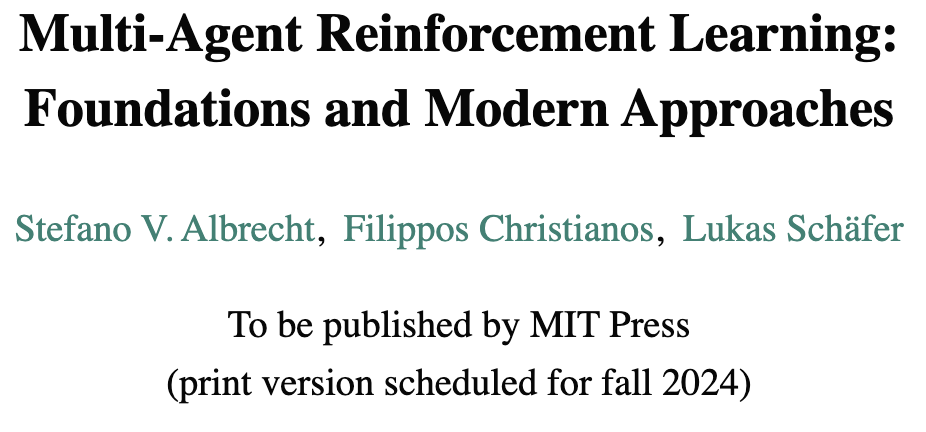
\includegraphics[width=\textwidth,height=.8\textheight,keepaspectratio]{images/1_MARL_book.png}
            
              \label{fig:enter-label}
            \end{figure}
          \end{column}
        
        \hspace{20pt}
            
          % Column for the text
            \begin{column}{0.45\textwidth}
	        \small

                This lecture is based on \textit{Multi-Agent Reinforcement Learning: Foundations and Modern Approaches} by Stefano V. Albrecht, Filippos Christianos and Lukas Sch\"afer
                
                \vspace{20pt}
                
                The book can be downloaded for free at \textcolor{blue}{\href{https://www.marl-book.com/}{www.marl-book.com}}.
            \end{column}
        
        \end{columns}
    \end{frame}
}

\newcommand{\leoslide}{
  \author{Stefano V. Albrecht, Filippos Christianos, Lukas Sch\"afer \\ Slides by: Leonard Hinckeldey}
}

\newcommand{\otherslide}{
  \author{Stefano V. Albrecht, Filippos Christianos, Lukas Sch\"afer}
}
	
\title{Multi-Agent Reinforcement Learning}
\date{}

\hypersetup{
  pdfsubject = {Multi-Agent Reinforcement Learning},
}

\leoslide

\subtitle{Introduction}

\begin{document}
\maketitle

\introslide

\begin{frame}{\outline}
    \vspace{10pt}
    \fat{Part 1: Introduction} 
    \vspace{5pt}
    \blist
        \item Multi-agent systems
        \item Advantages of MARL vs SARL in multi-agent systems
        \item Challenges of MARL   
    \elist
    \vspace{10pt}
    \fat{Part 2: Reinforcement Learning Basics} 
    \vspace{5pt}
    \blist
        \item Markov decision processes
        \item Discounted returns
        \item Dynamic programming and temporal-difference learning
    \elist
\end{frame}

\section{Part 1: Introduction}

\begin{frame}{What is MARL?}
		\textbf{\textit{Multi-agent reinforcement learning (MARL) is about finding optimal decision policies for two or more artificial agents interacting in a common environment.}}
  \vspace{20pt}
  \blist
    \item Applying reinforcement learning (RL) algorithms to multi-agent systems
    \item Goal is to learn optimal policies for two or more agents
  \elist
\end{frame}

\begin{frame}[t]{MARL Applications}
    \centering
    % Top left image
    \begin{minipage}{.5\linewidth}
        \centering
        
\includegraphics[width=.65\linewidth, keepaspectratio]{images/1_starcraft.png}
        
        Competitive games
    \end{minipage}%
    % Top right image
    \begin{minipage}{.5\linewidth}
        \centering
        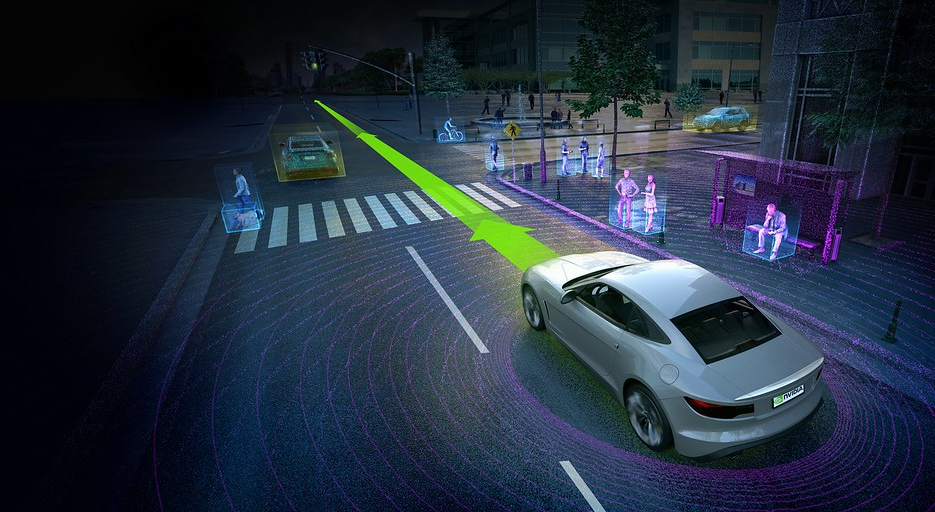
\includegraphics[width=.7\linewidth, keepaspectratio]{images/1_self_driving.png}
        
        Autonomous driving
    \end{minipage}
    
    % Bottom left image
    \begin{minipage}{.5\linewidth}
        \centering
        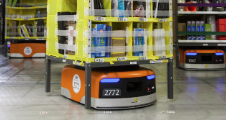
\includegraphics[width=.65\linewidth, keepaspectratio]{images/1_reware.png}
        
        Multi-robot warehouses
    \end{minipage}%
    % Bottom right image
    \begin{minipage}{.5\linewidth}
        \centering
        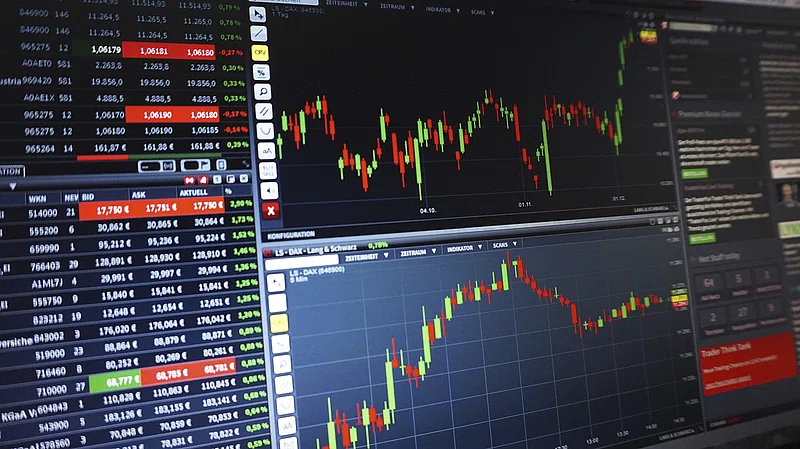
\includegraphics[width=.65\linewidth, keepaspectratio]{images/1_trading.png}
        
        Automated trading
    \end{minipage}

\end{frame}

\begin{frame}{Mutli-Agent Systems}
	\begin{graytitlebox}{A multi-agent system consists of:}
    \blist
        \item \textbf{Environment:} The environment is a physical or virtual world whose state evolves and is influenced by the agents' actions within the environment. 
        \item \textbf{Agents:} An agent is an entity which receives information about the state of the environment and can choose actions to influence the state.
        \listtab Agents are goal-directed, e.g. maximizing returns
    \elist
    \end{graytitlebox}
\end{frame}

% Need to edit potentially using columns. 
\begin{frame}{Multi-Agent Systems}		
    \begin{figure}
        \centering
        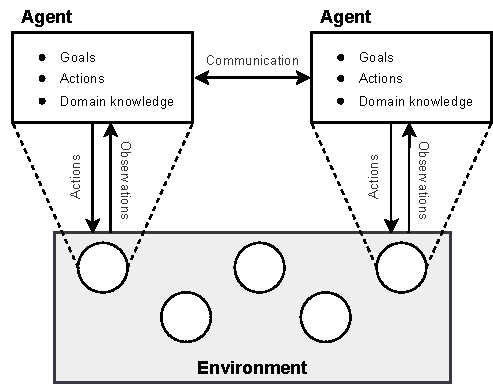
\includegraphics[width=\textwidth,height=.9\textheight,keepaspectratio]{images/chapter_1/mas_schematic.pdf}
        \label{fig:enter-label}
    \end{figure}
\end{frame}

\begin{frame}{Example: Level-Based Foraging}
	\bcol
		\col{0.5}
		    \blist
		        \item Three agents with varying skill levels
		        \item Goal: to collect all apples
		        \item Items can be collected if a group of one or more agents are located next to the item and the sum of agents' levels is greater than or equal to the item level
		        \item Action space $\Ac = \{up, down, left, right, collect, noop\}$
		    \elist
    	\col{0.45}
    		\centering
 	        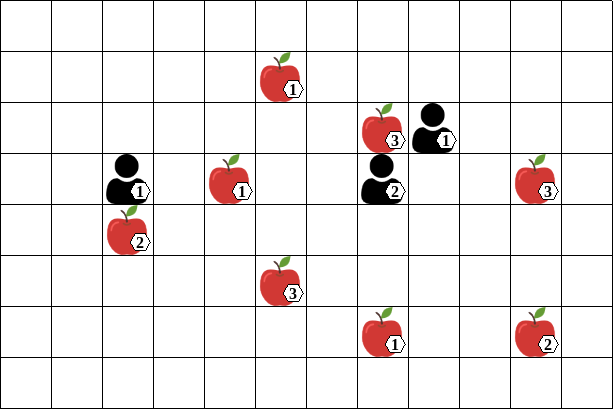
\includegraphics[width=\textwidth]{images/environments/lbf/foraging_8x12_b.png}
 	 \ecol
\end{frame}

\begin{frame}{MARL for Solving Multi-Agent Systems}

    \begin{figure}
        \centering
        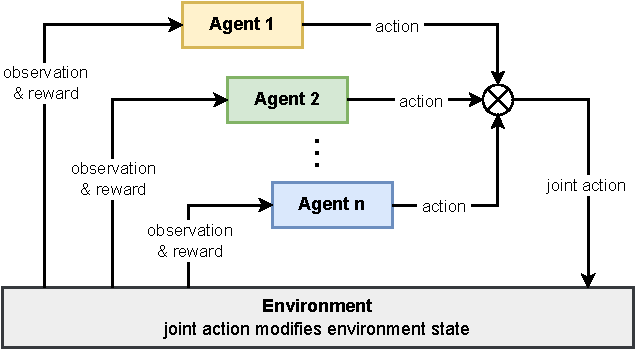
\includegraphics[width=.6\textwidth]{images/chapter_1/MARL-loop.pdf}
    \end{figure} 

    \blist
        \item Goal: learn optimal policies for a set of agents in a multi-agent system
        \item Each agent chooses an action based on its policy $\Rightarrow$ joint action
        \item Environment transitions into new state; agents receive rewards $+$ new observations
     \elist
\end{frame}

\begin{frame}{Why MARL?}
	\small

	Why should we use MARL to find optimal solutions to multi-agent systems rather than controlling multiple 'agents' using a single-agent RL (SARL) algorithm?% I.e. one agent controlling the actions of all agents. 

	\vspace{1.5em}

  \bcol
    \tcol{0.45}
    	\visible<2->{
        \e{Decomposing a larger problem}
        \blist
            \item For example, controlling $3$ agents each with $6$ actions (see LBF example), the action space becomes $6^3 = 216$.
            \item Using MARL, we decompose this into three more tractable problems. 
        \elist}

    \tcol{0.45}
	    \visible<3->{
        \e{Decentralized decision making}
        \blist
            \item There are many real-world scenarios where it is beneficial for each agent to make decisions independently.
            \item E.g. autonomous driving is impractical for frequent long-distance data exchanges between a central agent and the vehicle.
        \elist}
	\ecol
\end{frame}

\begin{frame}{Challenges of MARL}
	\begin{graytitlebox}{New \fat{challenges} arise in MARL:}
    \blist
        \item<1-> Non-stationarity caused by multiple learning agents
        \item<2-> Optimality of policies and equilibrium selection
        \item<3-> Multi-agent credit assignment
        \item<4-> Scaling in number of agents
    \elist
    \end{graytitlebox}
    
    We will explore these challenges in upcoming lectures!
    
\end{frame}

% \begin{frame}{MARL Applications of }

%     \fat{Competitive Gaming:}
%     \blist
%         \item Video and Board Games (Backgammon, Chess, Go, Starcraft etc.).
%     \elist
%     \fat{Warehousing:}
%     \blist
%         \item Warehouse Robot Management, robots that can 
%         retrieve items requested by users from the warehouse).
%     \elist
%     \fat{Autonomous Driving:}
%     \blist
%         \item Autonomous Driving (controlling policies for multiple vehicles to navigate through complex interaction. 
%     \elist
%     \fat{Trading Bots:}
%     \blist
%         \item Automated Trading in Electronic Markets.
%     \elist
    
% \end{frame}

\section{Part 2: Reinforcement Learning Basics}


\begin{frame}{Back to RL Basics}

    \begin{figure}
        \centering
        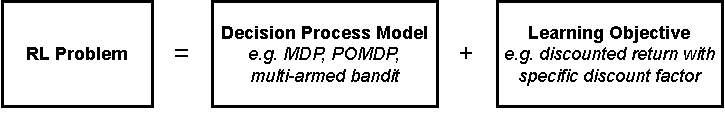
\includegraphics[width=0.9\textwidth]{images/chapter_2/rl-learning-problem.pdf}
    \end{figure}

    \blist
        \item RL algorithms learn solutions for sequential decision problems via repeated environment \textbf{interaction}
        \item Sequential decision process is defined formally as \e{Markov decision process} (MDP)
        \item Goal is to learn an optimal decision policy for a specific learning objective
    \elist
    
\end{frame}

\begin{frame}{MDP As a Graph}
    
      \centering
      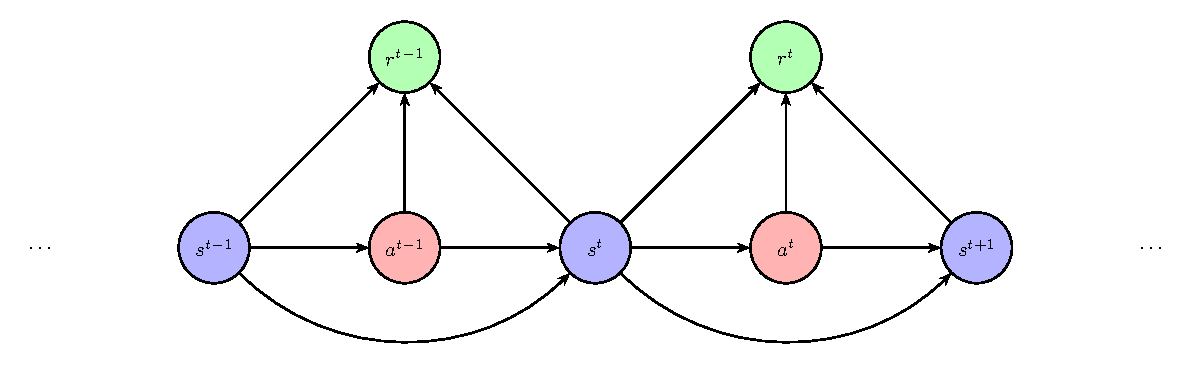
\includegraphics[width=1\textwidth]{images/1_mdp_diagram_elipses.pdf}
    
\end{frame}

\begin{frame}{MDP Definition}
  \bcol

    % Left column for text
    \col{0.5}
     MDP is defined as a tuple $(S, A, \mathcal{R}, \mathcal{T}, \mu):$
     
      \blist
        \item \textcolor{blue}{$S$}: Finite set of states with subset of terminal states $\bar{S} \subset S$
        \item \textcolor{red}{$A$}: Finite set of actions
        \item \textcolor{green}{$\mathcal{R}$}: Reward function $\mathcal{R}: \textcolor{blue}{S} \times \textcolor{red}{A} \times \textcolor{blue}{S} \to \mathbb{R}$
        \item $\mathcal{T}:$ State transition function $\mathcal{T}: \textcolor{blue}{S} \times \textcolor{red}{A} \times \textcolor{blue}{S} \to [0, 1]$
        \item $\mu$: Initial state distribution $\mu: S \to [0,1]$ such that $\sum_{s\in S}\mu (s) = 1$ and $\forall s \in \hat{S}: \mu (s) = 0$
      \elist

    \col{0.5}
        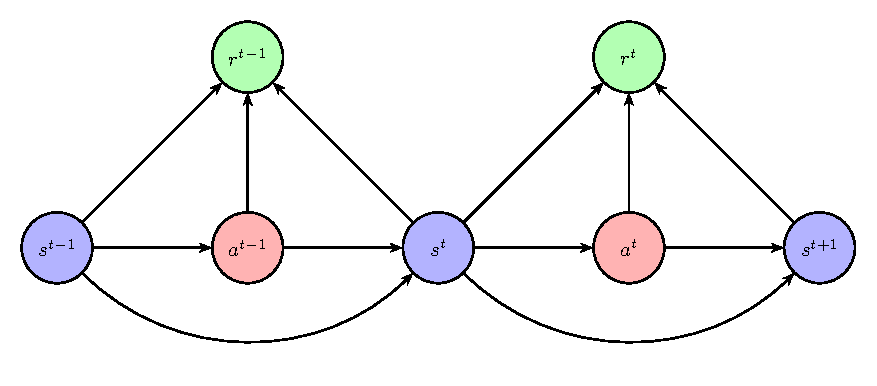
\includegraphics[width=\linewidth]{images/1_mdp_diagram.pdf}

  \ecol
\end{frame}

\begin{frame}{MDP Assumptions}

    \begin{columns}[T]
        \begin{column}{0.5\textwidth}
        	\visible<1->{
            \fat{\e{Markov property}}
            \blist
                \item Future states are temporally independent of past states and actions, given the current state and action. 
                \item $Pr(s^{t+1}, r^{t}|s^{t}, a^{t}, s^{t-1}, a^{t-1}, ...,s^0, a^0) = Pr(s^{t+1}, r^{t}|s^{t}, a^{t})$
                % \item Meaning that the current state provides all necessary information for an agent to choose the optimal action. 
            \elist }
            \vspace{10pt}
            \visible<2->{
            \fat{\e{Full observability}}
            \blist
                \item The agent can see the entire state of the environment. 
                \item In practice, agent may only have partial view.
            \elist} 
        \end{column}
        
        \hspace{10pt}
        
        \begin{column}{0.5\textwidth}
            \visible<3->{
            \fat{\e{Stationarity}}
            \blist
                \item The dynamics of the environment are assumed to be stationary. 
                \item i.e. $\mathcal{T}$ and \textcolor{green}{$\mathcal{R}$} remain constant through time. 
            \elist}
            \vspace{10pt}
            \visible<4->{
            \fat{\e{Incomplete knowledge of MDP}}
            \blist
                \item The agent may only have knowledge of the action and state spaces ($\textcolor{red}{A}, \textcolor{blue}{S}$)
                \item The transition and reward function ($\mathcal{T}, \mathcal{R}$) are usually to be \fat{unknown}.
            \elist}
        \end{column}
    \end{columns}
\end{frame}

\begin{frame}{Mars Rover MDP Example}
    \begin{columns}[onlytextwidth] 
    
      \begin{column}{0.5\textwidth}
        \begin{figure}
          \centering
          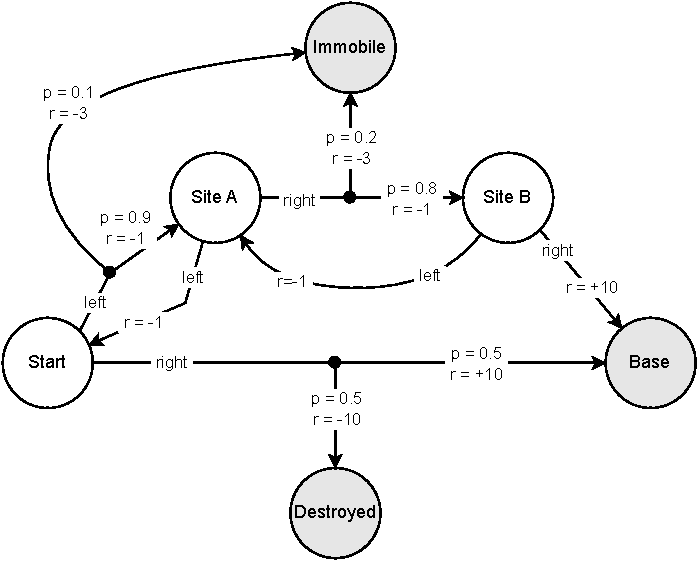
\includegraphics[width=\textwidth,height=.8\textheight,keepaspectratio]{images/chapter_2/mdp-rover.pdf}
          \label{fig:enter-label}
        \end{figure}
      \end{column}
    
      % Column for the text
      \begin{column}{0.5\textwidth}
        \blist
          \item \textit{Start} is the initial state \(s^0\)
          \item Two possible actions \(A = \{right, left\}\)
          \item Goal is to get to \textit{Base}
          \item Rewards given by $\mathcal{R}(s, a, s')$ are shown as $r$. 
          \item State transition probabilities given by $\mathcal{T}(s, a, s)$, are shown as $p$
        \elist
      \end{column}
    
    \end{columns}
\end{frame}

\begin{frame}{RL for Optimizing Policies in MDPs}

        \centering
        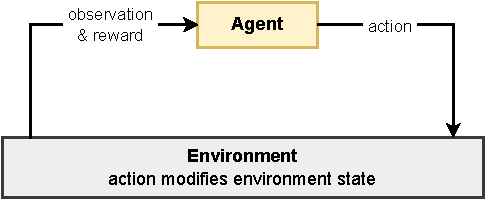
\includegraphics[width=0.6\textwidth]{images/chapter_2/RL-loop.pdf}

	\vspace{2em}

    \bcol
        \col{0.47}
            \e{\fat{Value-Based RL}} \\
            These methods indirectly update the policy by learning value functions.

        \col{0.47}
            \e{\fat{Policy-Based RL}} \\
            These methods update a parameterized policy function directly.
                % \item These methods also include hybrid approaches (actor-critic) that update a parameterised policy function but use value function approximation as a baseline. 
    
    \ecol
    
\end{frame}

\begin{frame}{Expected Discounted Returns}

    Using RL, we aim to maximize the expected \textbf{return}.

    \blist
        \item Returns ($u$) are the sum of rewards received over time
        \item If MDP is non-terminating (i.e. $t \to \infty$), we \textbf{discount} returns to ensures finite (discounted) returns
    \elist
    \vspace{0pt}
    $$
    \mathbb{E}_{\pi}[u_{t}] = \mathbb{E}_{\pi}\left[\sum_{t=0}^{\infty}\gamma^t r^t\right]
    $$

    \blist
        \item $\gamma$ is the discount factor, such that $\gamma \in [0, 1]$
        \item $\pi$ is the behavior policy that determines which actions are chosen.
    \elist
\end{frame}

\begin{frame}{State-Value Functions}

    \textbf{State-value} functions $V^{\pi}(s)$ give the 'value' of state $s$ when following the policy $\pi$. 
    \vspace{0pt}
    \begin{align*}
    V^{\pi}(s) = \mathbb{E}_\pi \left[u^{t} | s^{t} = s \right]
    \end{align*}
    \vspace{0pt}
    The return ($u$) can be recursively defined as:
    \vspace{0pt}
    \begin{align*}
            u^t &= r^t +\gamma (r^{t+1} + \gamma r^{t+2} + ... )  \\ &= r^t + \gamma u^{t+1}
    \end{align*}
    \vspace{0pt}   
    Therefore:
    \vspace{0pt}
    \begin{align*}
        V^{\pi}(s) = \mathbb{E}_\pi \left[r^t + \gamma u^{t+1}| s^{t} = s \right]
    \end{align*}
    \vspace{5pt}
\end{frame}

\begin{frame}[t]{The Bellman Equation}

    \begin{align*}
        V^{\pi}(\st) &= \ex{\pi}{\rew^t + \gamma u^{t+1} \mid \st^{t} = \st } \\[3pt]
                   &= \sum_{\ac \in \Ac} \pi(\ac \mid \st) \sum_{\st' \in \St} \Stf(\st'\mid \st, \ac) \left[\Rew(\st, \ac, \st') + \gamma \ex{\pi}{u^{t+1} \mid \st^{t+1} = \st'}\right] \\[3pt]
                   &= \sum_{\ac \in \Ac} \pi(\ac \mid \st) \sum_{\st' \in \St} \Stf(\st'\mid \st, \ac) \left[\Rew(\st, \ac, \st') + \gamma V^{\pi}(\st')\right]
    \end{align*}
    
    The last equation is known as the \e{Bellman equation} in honor of Richard Bellman. 
    
    \blist
        \item The value of being in state $s$ while following a fixed policy $\pi$ is equivalent to the immediate reward ($\Rew(\st, \ac, \st') \to \rew$) received when taking action $\ac$ in state $\st$ ($\pi(\ac \mid \st)$) plus the discounted value of the next state $\st'$. 
    \elist
\end{frame}

\begin{frame}{State-Action Value Function}
    \textit{State-Action} value functions $Q^{\pi}(s,a)$ are an extension on the \textit{State} value functions. They condition the expected return on the current state and the action taken.
    \begin{align*}
         Q^{\pi}(s,a) = \mathbb{E}_{\pi}\left[u^{t}|s^{t}=s, a^{t}=a\right]
    \end{align*}

The \textit{state-action} value Bellman equation is therefore:
\vspace{10pt}
\begin{align*}
    Q^{\pi}(s,a) = \sum_{a \in A} \pi(a|s) \sum_{s' \in S} \mathcal{T}(s'|s,a) \left[\mathcal{R}(s,a,s') + \gamma Q^{\pi}(s')\right]
\end{align*}

\end{frame}

\begin{frame}{Greedy Policies}

    A policy can act \textit{greedily} i.e. choosing actions which maximize the immediate reward and the value of the next state.
    \vspace{10pt}
    
    Greedy $\pi$ using \textit{state value} functions:
    \vspace{5pt}    
    \begin{align*}
       \pi(s) = \argmax_{a \in A} \sum_{s', r} \mathcal{T}(s', r | s, a) \left[ r + \gamma V(s') \right]
    \end{align*}
    
    Or using the \textit{state-action value function}:
    \vspace{5pt}
    \begin{align*}
        \pi(s) = \argmax_{a \in A}Q(s, a)    
    \end{align*}
    
\end{frame}

\begin{frame}{Optimal Greedy Policy}

   A greedy policy with respect to a value function is optimal only when using the \textbf{optimal value function.} 
    
    An \textbf{optimal value function} for a MDP can be defined as:
    \vspace{5pt}
    \begin{align*}
        V^{*}(s) &= \max_{\pi'} V^{\pi'}(s), \quad \forall s \in S \\
        Q^{*}(s, a) &= \max_{\pi'} Q^{\pi'}(s, a), \quad \forall s \in S, a \in A
    \end{align*}

    Therefore, the optimal policy is:
    \vspace{5pt}
    \begin{align*}
        \pi^{*}(s) = \argmax_{a \in A}Q^{*}(s, a)    
    \end{align*}
\end{frame}

\begin{frame}{Dynamic Programming}
    \blist
        \item Dynamic Programming (DP) is a family of algorithms to compute \textbf{optimal value functions} and \textbf{optimal policies in MDPs} (Bellman 1957; Howard 1960).
        \item In DP, we \textbf{assume complete knowledge} of the MDP, including the transition and reward function ($\mathcal{T}, \mathcal{R}$).
        \item Given complete knowledge, we can use the \textbf{Bellman equation} to find optimal value functions and policies.
    \elist   
\end{frame}

\begin{frame}{Policy Iteration}
    \fat{Policy iteration} is a DP algorithm that alternates between two steps:
        \blist
            \item \textbf{Policy evaluation}: compute value function $V^{\pi}$ for current policy $\pi$
            \item \textbf{Policy improvement}: improve current policy $\pi$ with respect to $V^{\pi}$
        \elist 

    \begin{align*}
        \pi^{0} \to V^{\pi^{0}}\to \pi^{1} \to V^{\pi^{1} } \to\pi^{2} \to ... \to V^{*} \to \pi^{*} 
    \end{align*}

    % \begin{figure}
    %     \centering
    %     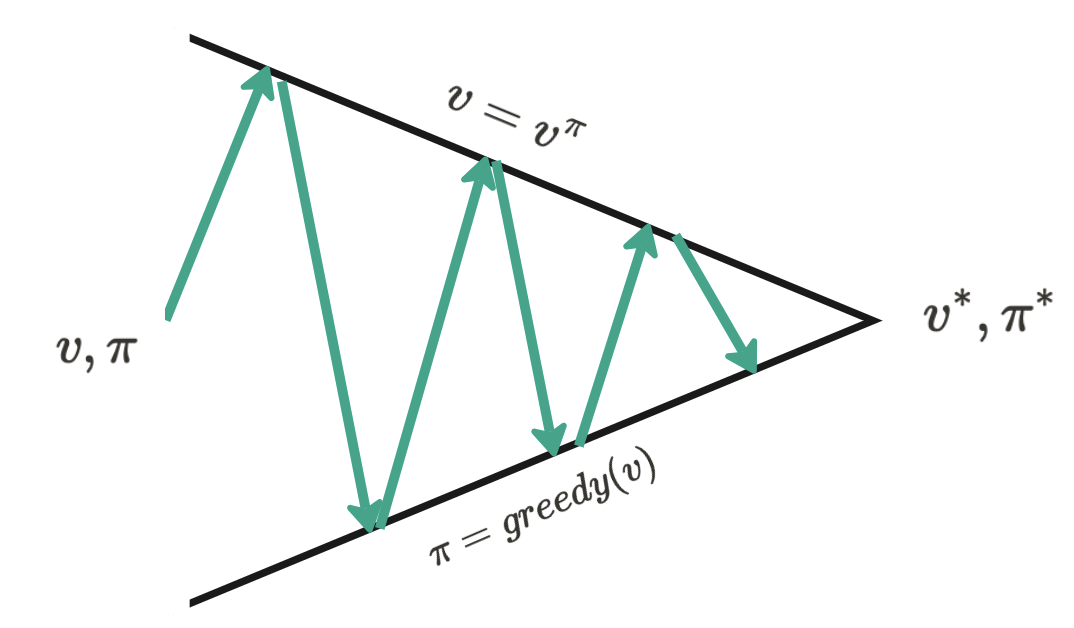
\includegraphics[width=\textwidth,height=.45\textheight,keepaspectratio]{images/1_policy_iteration.png}
    %     \label{fig:policy_iteration}
    % \end{figure}
\end{frame}

\begin{frame}[fragile]{Policy Iteration Pseudo Code}
\centering
\scalebox{0.8}{\begin{minipage}{\linewidth}
    \balg{Policy Iteration}{pi}
        \State Initialize $\pi$ randomly, initialise $V(s)$ arbitrarily for all $s \in S$ except $V(\text{terminal}) = 0$
        \Repeat
            \State \textbf{Policy Evaluation:}
            \Repeat
                \For{each state $s$ in $S$}
                    \State $V(s) \gets \sum_{s'} \mathcal{T}(s' | s, \pi(s)) [\mathcal{R}(s, \pi(s), s') + \gamma V(s')]$
                \EndFor
            \Until{$V(s)$ converges for all $s \in S$}
            \State \textbf{Policy Improvement:}
            \State policy\_stable $\gets$ true
            \For{each state $s$ in $S$}
                \State old\_action $\gets \pi(s)$
                \State \Cboxed{red}{$\pi(s) \gets \arg\max_a \sum_{s'} \mathcal{T}(s' | s, a) [\mathcal{R}(s, a, s') + \gamma V(s')]$}
                \If{old\_action $\neq \pi(s)$}
                    \State policy\_stable $\gets$ false
                \EndIf
            \EndFor
        \Until{policy\_stable}
        \Return $V, \pi$
    \ealg
\end{minipage}%
    }
\end{frame}


\begin{frame}{Value Iteration}
	\textbf{Value Iteration} uses the \textbf{Bellman optimality equation}
    \blist
        \item Combines iterative policy evaluation and improvement into one single update equation.
    \elist

    \textit{Bellman Optimality Equation as update operator:}
    \begin{align*}
        V^{k+1}(s) \gets \max_{a \in A} \sum_{s' \in S} \mathcal{T}(s' | s, a) [\mathcal{R}(s, a, s') + \gamma V^k(s')], \quad \forall s \in S
    \end{align*}

    \blist
        \item The max operator makes this the Bellman \textit{optimality} equation.
        \item The equation expresses the value of a state as the maximum expected return achievable by taking the best action and then following the optimal policy.
    \elist
\end{frame}

\begin{frame}[fragile]{Value Iteration Pseudo Code}

    \balg{Value Iteration}{vi}
        \State Initialize: $V(s) = 0, \forall s \in S$
        \Repeat
            \State \Cboxed{red}{$\forall s \in S: V(s) \gets \max_{a \in A} \sum_{s' \in S} \mathcal{T}(s' | s, a) \left[\mathcal{R}(s, a, s') + \gamma V(s')\right]$}
        \Until{$V$ converged}
        \Return{ optimal policy $\pi^{*}$ with:}
        \State $\forall s \in S: \argmax_{a \in A} \sum_{s' \in S}\mathcal{T}(s'|s, a)\left[\mathcal{R}(s, a, s')+\gamma V(s') \right]$
    \ealg

\end{frame}

\begin{frame}{Temporal-Difference Learning}
    \textbf{Temporal-Difference} (TD) learning is a family of RL algorithms that learn optimal policies and value functions based on data collected via environment \textbf{interactions}. 

    \blist
        \item These algorithms learn which actions yield the best returns by 
        \textbf{trial and error} and exploring different actions and states
    	\listtab Learns without \textbf{model} of environment's \textbf{reward} and \textbf{transition} functions ($\mathcal{R}, \mathcal{T}$)
        \listtab Can learn \textbf{online}, updating the policy while interacting with the environment
    \elist
\end{frame}

\begin{frame}{Temporal Difference Update}
    The update for temporal-difference learning relies on value functions:
    \vspace{0pt}
    \begin{align*}
        V(s^{t}) \gets V(s^{t}) + \alpha \left[\mathcal{X} - V(s^{t})\right]
    \end{align*}
    or 
    \vspace{0pt}
    \begin{align*}
        Q(s^{t}, a^{t}) \gets (s^{t}, a^{t})  + \alpha \left[\mathcal{X} - (s^{t}, a^{t})\right]
    \end{align*}
	\blist
    	\item $\mathcal{X}$ is the update target, serving as an estimate of the current state value. 
    	\item $\alpha$ is the learning rate
    \elist
\end{frame}

\begin{frame}{Temporal-Difference Update}
    
    In SARSA (a basic TD algorithm), we use the experience tuple $(\st^{t}, \ac^{t}, \rew^{t}, \st^{t+1}, \ac^{t+1})$ to construct a target:
    \vspace{10pt}
    \begin{align*}
        \mathcal{X} = \rew^t + \gamma Q(\st^{t+1}, \ac^{t+1})
    \end{align*}
    
    (The immediate reward plus the discounted value of the next state) - note the resemblance to the Bellman equation. 
    \vspace{10pt}
    \begin{align*}
        Q^{\pi}(\st, \ac) = \sum_{\ac \in \Ac} \pi(\ac \mid \st) \sum_{\st' \in \St} \Stf(\st' \mid \st, \ac) \Cboxed{red}{$\left[\Rew(\st, \ac, \st') + \gamma Q^{\pi}(s', a')\right]$}
    \end{align*}
\end{frame}

\begin{frame}{SARSA}
    
The SARSA update rule thus becomes:
\vspace{0pt}
\begin{align*}
  Q(s^t, a^t) \leftarrow Q(s^t, a^t) + \alpha[r^t + \gamma Q(s^{t+1}, a^{t+1})- Q(s^t,a^t)] 
\end{align*}

\blist
    \item Note the TD error $r^t + \gamma Q(s^{t+1}, a^{t+1})- Q(s^t,a^t)$.
    \item The TD update is \textbf{bootstrapped}
    \item Using the value \textbf{estimates} of the next state ($Q(s^{t+1}, a^{t+1})$) to update the current state value ($Q(s^t,a^t)$)
\elist



\end{frame}

\begin{frame}[fragile]{SARSA Pseudo Code}
    \centering 
    \balg{SARSA}{sarsa}
        \State Initialize \( Q(s, a) = 0 \) for all \( s \in S, a \in A \)
        \For{every episode}
            \State Observe initial state \( s^0 \)
            \State With probability \( \epsilon \): choose random action \( a^0 \in A \)
            \State Otherwise: choose action \( a^0 \in \arg\max_a Q(s^0, a) \)
            \For{\( t = 0, 1, 2, \ldots \)}
                \State Apply action \( a^t \), observe reward \( r' \) and next state \( s^{t+1} \)
                \State With probability \( \epsilon \): choose random action \( a^{t+1} \in A \)
                \State Otherwise: choose action \( a^{t+1} \in \arg\max_a Q(s^{t+1}, a) \)
                \State \Cboxed{red}{\( Q(s^t, a^t) \gets Q(s^t, a^t) + \alpha [ r^{t} + \gamma Q(s^{t+1}, a^{t+1}) - Q(s^t, a^t) ] \)}
            \EndFor
        \EndFor
    \ealg
\end{frame}

\begin{frame}{Convergence of SARSA}

    SARSA is guaranteed to converge to the optimal \textbf{state-value function}, for all $S \in S$ and $a \in A$, if:
    \vspace{10pt}
    \blist
        \item All \textit{state-action} pairs are explored infinitely many times: $$\forall s \in S, a \in A: \sum_{k=0}^{\infty} \mathbb{I}(s, a) \to \infty $$
        \item The learning rate $\alpha$ is reduced over time according to the "standard stochastic approximation conditions": $$\forall s \in S, a \in A: \sum_{k=0}^{\infty} \alpha_k(s, a) \to \infty \quad \text{and} \quad \sum_{k=0}^{\infty} \alpha_k(s, a)^2 < \infty$$
    \elist        
\end{frame}

\begin{frame}{$\epsilon$-Greedy Policies}

    Using a \textbf{greedy policy} would \textbf{violate the convergence condition} of SARSA (infinite exploration of $S$ and $A$). 
    \vspace{0pt}
    \blist
        \item Intuitively, we must explore a wide range of states and actions to find state action combinations that yield high returns
        \item One solution is to add an \textbf{exploration} parameter $\epsilon \in [0, 1]$. This gives us a stochastic \textbf{epsilon-greedy} policy.
    \elist
    \vspace{0pt}
    \begin{align*}
        \pi(a|s) = \begin{cases} 
        1 - \epsilon + \frac{\epsilon}{|A|} & \text{if } a \in \arg\max_{a'} Q(s, a') \\
        \frac{\epsilon}{|A|} & \text{otherwise} 
    \end{cases}
    \end{align*}

    \blist
        \item With probability $1-\epsilon$, the policy chooses the greedy action, and with probability $\epsilon$ chooses an action uniformly at random. 
    \elist
    
\end{frame}

\begin{frame}{Q-Learning}

    \e{Q-learning} (Watkins \& Dayan 1992) is a popular TD algorithm which uses the Bellman optimality equation to update its value function estimates.
    \vspace{10pt}
    \blist
        \item By using the Bellman optimality equation, Q-learning directly learns the \textbf{optimal state-action value function}
        \item Q-learning is \textbf{off-policy}, meaning the policy followed to gather experiences is different from the optimized policy
        \item We use the $\epsilon$-greedy policy to collect experiences
    \elist

\end{frame}

\begin{frame}{Q-Learning Update}

    The target in Q-learning uses the \textit{max} operator to target the optimal Q-values directly. 
    \vspace{00pt}
    \begin{align*}
        \mathcal{X} = r^{t} + \gamma \max_{a' \in A}Q(s^{t+1}, a')
    \end{align*}

    The Q-learning update is thus:
    \vspace{0pt}
    \begin{align*}
        Q(s^t, a^t) \gets Q(s^t, a^t) + \alpha \left[ r^t + \gamma \max_{a' \in A} Q(s^{t+1}, a') - Q(s^t, a^t) \right]
    \end{align*}
    
\end{frame}

\begin{frame}{Q-Learning Pseudo Code}
    \centering
    \balg{Q-Learning}{ql}
        \State Initialize $Q(s, a) = 0$  for all $\st \in \St, \ac \in \Ac$
        \For{every episode}
            \For{$t = 0, 1, 2, \ldots$} 
                \State Observe current state $s^t$
                \State With probability $\epsilon$: choose random action $\ac^t \in \Ac$
                \State Otherwise: choose action $\ac^t \in \arg\max_{\ac} Q(\st^t, \ac)$
                \State Apply action $\ac^t$, observe reward $\rew^t$ and next state $\st^{t+1}$
                \State \Cboxed{red}{$Q(\st^t, \ac^t) \gets Q(\st^t, \ac^t) + \alpha \left[ \rew^t + \gamma \max_{\ac'} Q(\st^{t+1}, \ac') - Q(\st^t, \ac^t) \right]$}
            \EndFor
        \EndFor
    \ealg
\end{frame}


\begin{frame}{Evaluating RL Algorithms}

    \begin{columns}
    \begin{column}{0.5\textwidth}
        
        \begin{figure}
            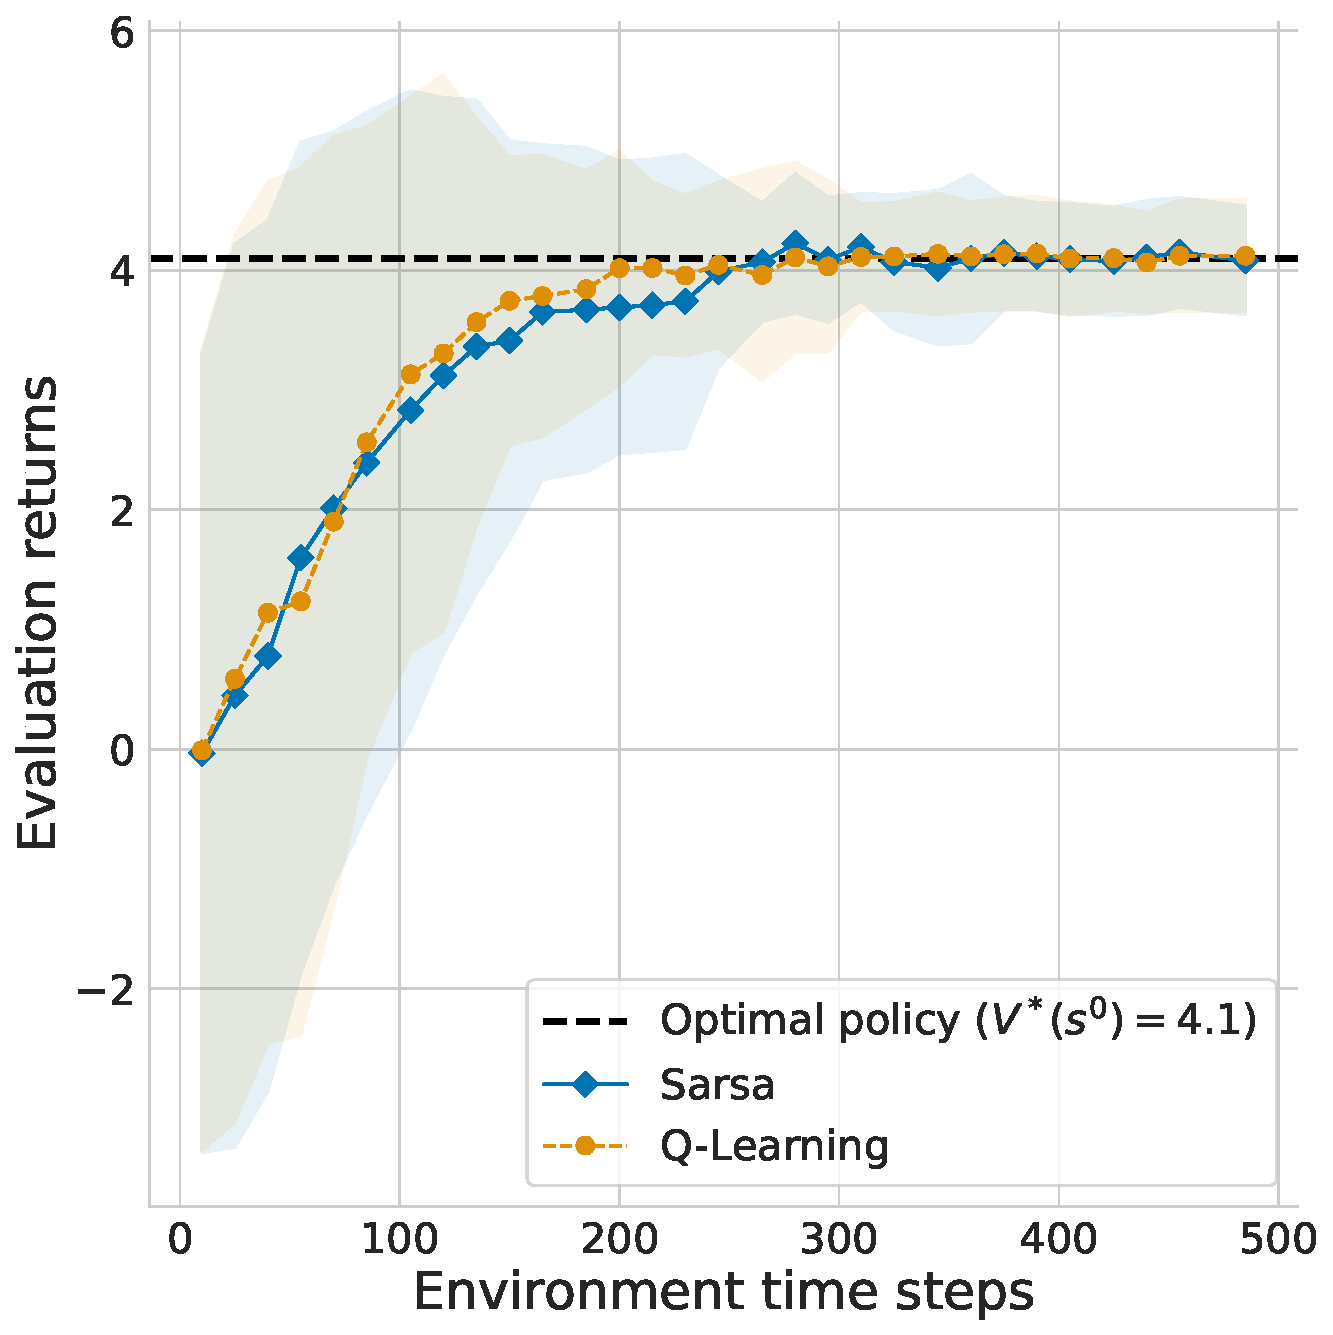
\includegraphics[width=0.45\linewidth, height=0.45\textheight, keepaspectratio]{images/chapter_2/tabular_mdp_returns.pdf}
            \hspace{5pt} % Horizontal space between images
            % Row 1, Image 2
            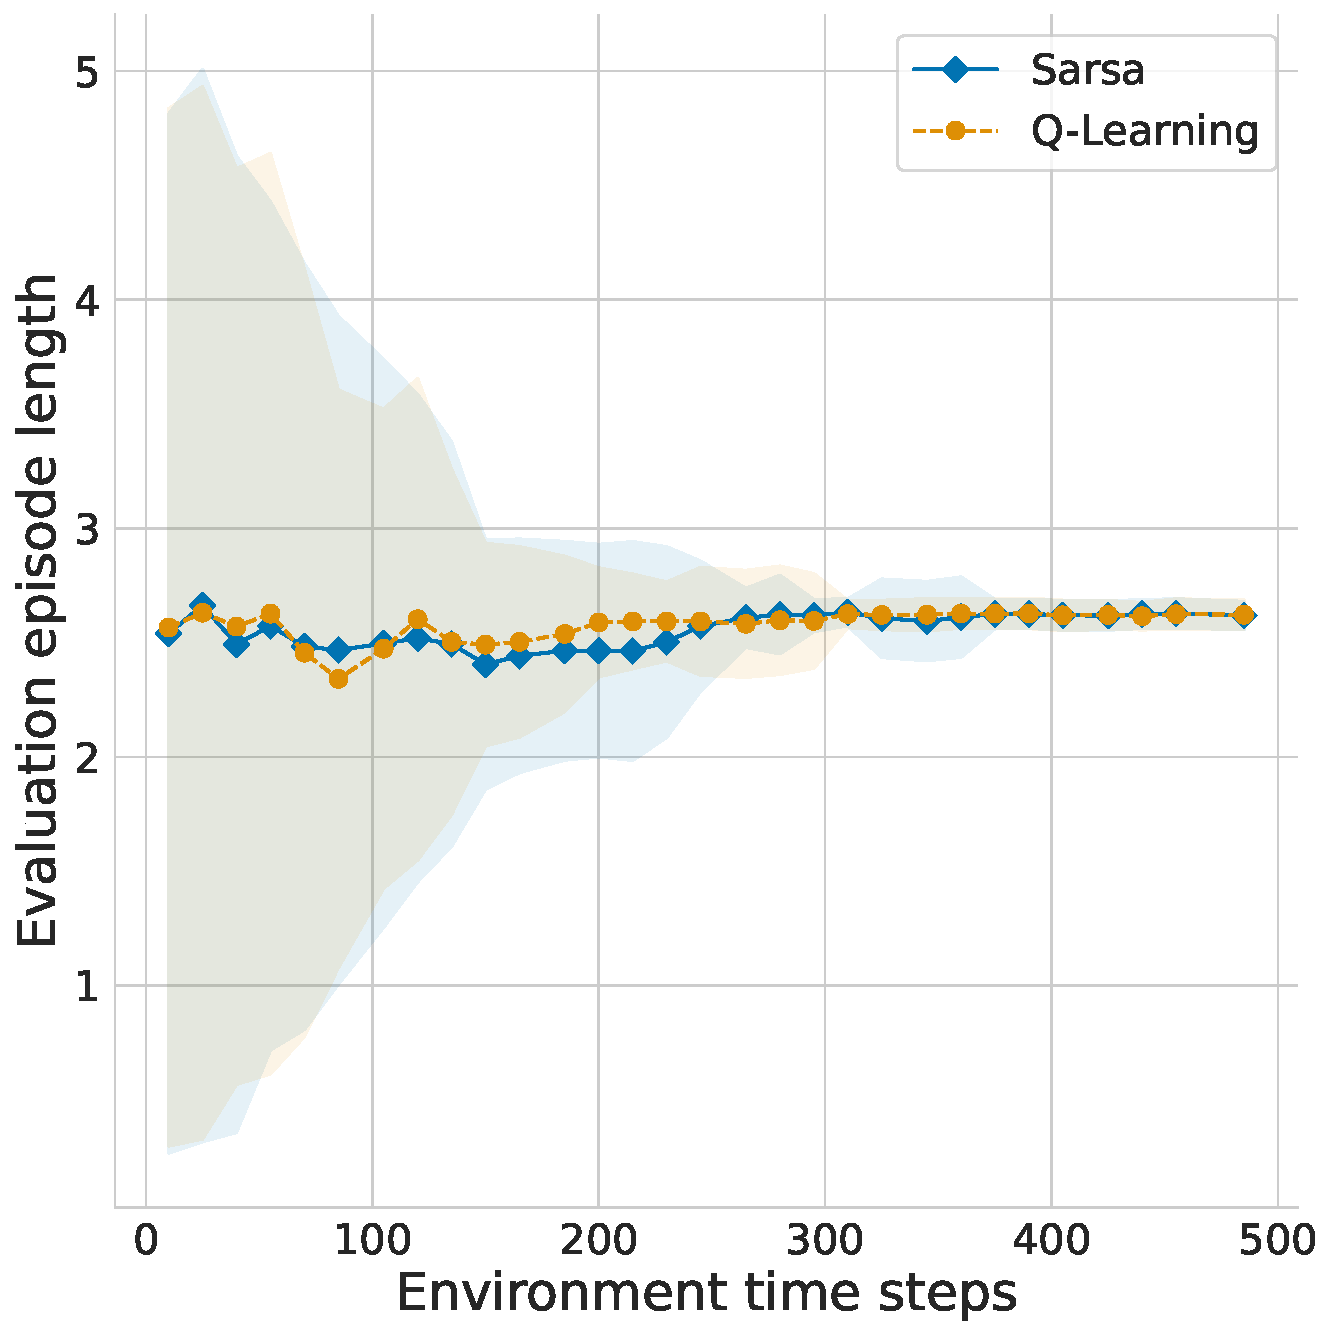
\includegraphics[width=0.45\linewidth, height=0.45\textheight, keepaspectratio]{images/chapter_2/tabular_mdp_eplength.pdf}
        
            \vspace{5pt} % Vertical space between rows
        
            % Row 2, Image 3
            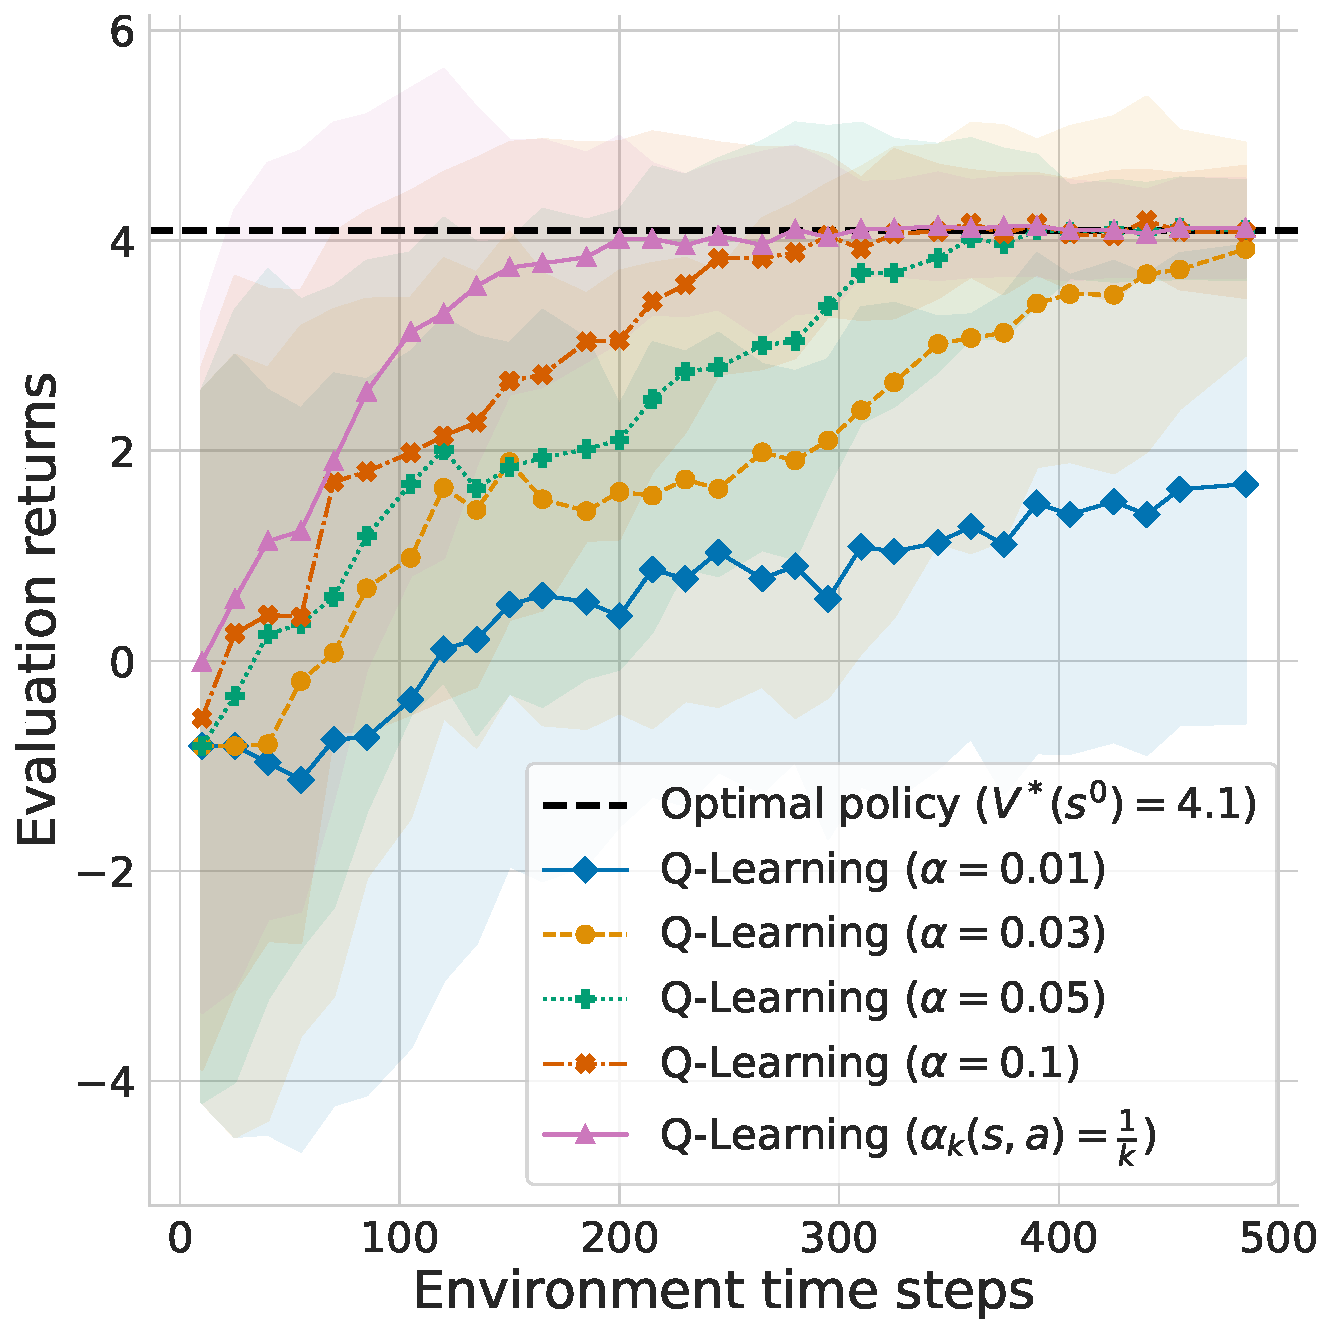
\includegraphics[width=0.45\linewidth, height=0.45\textheight, keepaspectratio]{images/chapter_2/tabular_mdp_ql_alphas_returns.pdf}
            \hspace{5pt} % Horizontal space between images
            % Row 2, Image 4
            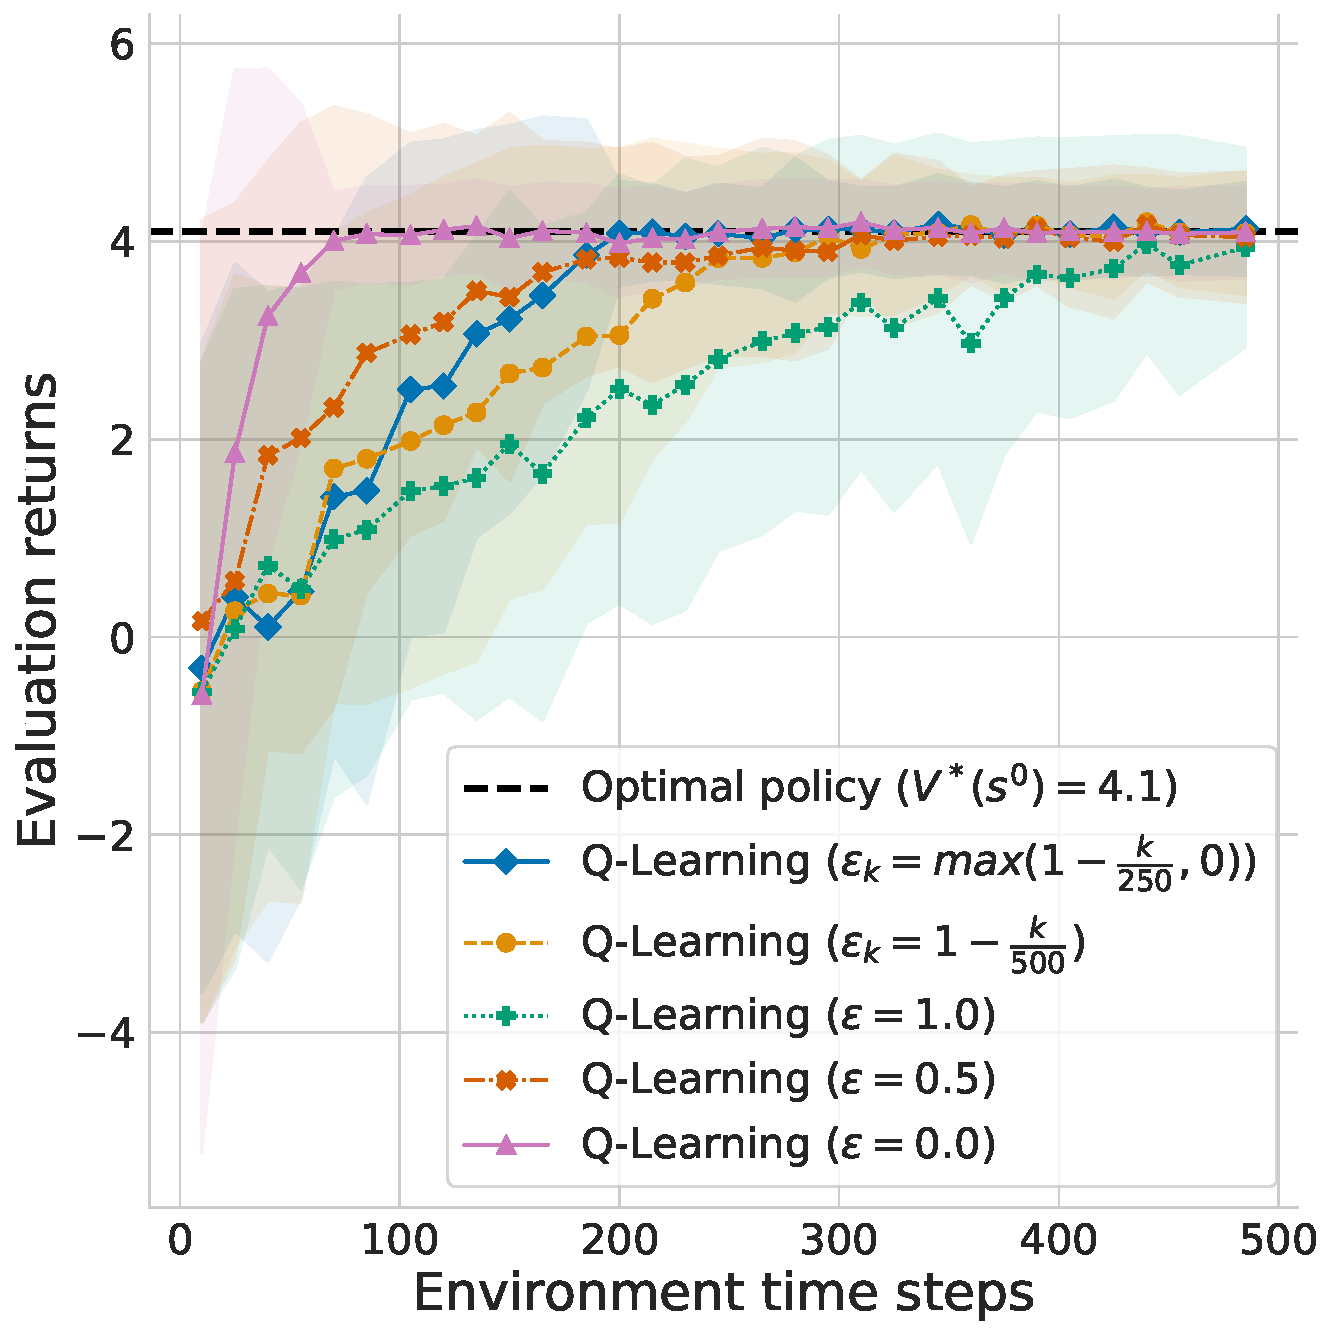
\includegraphics[width=0.45\linewidth, height=0.45\textheight, keepaspectratio]{images/chapter_2/tabular_mdp_ql_eps_returns.pdf}
        \end{figure}
        \end{column}
        \begin{column}{0.5\textwidth}
            
            \textbf{Y-axis:}

            \blist
                \item {\small Average \textbf{discounted evaluation returns}. This shows us how our greedy policy would perform if we stopped learning at time step T.} 
                \item {\small In some cases, \textbf{undiscounted returns} are easier to interpret and may be used instead. }
            \elist
            
            \textbf{X-axis:}
            \blist 
                \item {\small Cumulative training steps across episodes.} 
                \item {\small Number of episodes can also be used. This might, however, distort the learning speed.} 
            \elist
        \end{column}
        
    \end{columns}

\end{frame}

% \begin{frame}{Evaluating RL Algorithms Continued}
% \small
%   \begin{columns}[T]
%     \begin{column}{0.6\textwidth}
%         \fat{Why Cumulative Time Steps and not n Episodes?}
%         \blist
%             \item Episodes can distort the speed at which an algorithm learns. 
%             \item Maybe, and the algorithm needs a few episodes to converge, but it takes a lot of time to explore in early episodes. 
%         \elist
        
%         \fat{Average Discounted Evaluation Returns.}
%         \blist
%             \item Returns are from a greedy policy with respect to learned action values after T time steps. 
%             \item We average to answer the following question: if we finish learning after T time steps and extract the greedy policy, what expected returns can we expect to achieve with this policy?
%         \elist
%     \end{column}

%     \begin{column}{0.4\textwidth}
%         \fat{What about Undiscounted Returns?}
%         \blist
%             \item We usually use discounted returns as this is the learning objective, but undiscounted rewards can sometimes be easier to interpret. 
%             % \item For example, suppose we want to learn an optimal policy for a video game in which the agent controls a spaceship and receives a +1 score (reward) for each destroyed enemy. If in an episode the agent destroys 10 enemies at various points in time, the undiscounted return will be 10 but the discounted return will be less than 10, making it more difficult to understand how many enemies the agent destroyed.
%         \elist
%     \end{column}

%   \end{columns}

% \end{frame}

\begin{frame}{Summary}

\fat{We covered:}
\blist
    \item Multi-Agent Systems and the case for MARL
    \item MDPs
    \item Value Functions
    \item Dynamic Programming
    \item Temporal Difference Learning (SARSA and Q-Learning)
\elist
\fat{Next we'll cover:}
\blist
    \item Games: Models of Multi-Agent Interaction
\elist

\end{frame}

\begin{frame}{Reading}

Richard Bellman: Dynamic Programming. Princeton University Press, 1957

Ronald Howard: Dynamic Programming and Markov Processes. John Wiley, 1960

Richard Sutton and Andrew Barto: Reinforcement learning: An introduction (2nd edition). MIT Press, 2018

\end{frame}
\end{document}
